\documentclass[]{article}
\usepackage{lmodern}
\usepackage{amssymb,amsmath}
\usepackage{ifxetex,ifluatex}
\usepackage{fixltx2e} % provides \textsubscript
\ifnum 0\ifxetex 1\fi\ifluatex 1\fi=0 % if pdftex
  \usepackage[T1]{fontenc}
  \usepackage[utf8]{inputenc}
\else % if luatex or xelatex
  \ifxetex
    \usepackage{mathspec}
  \else
    \usepackage{fontspec}
  \fi
  \defaultfontfeatures{Ligatures=TeX,Scale=MatchLowercase}
\fi
% use upquote if available, for straight quotes in verbatim environments
\IfFileExists{upquote.sty}{\usepackage{upquote}}{}
% use microtype if available
\IfFileExists{microtype.sty}{%
\usepackage{microtype}
\UseMicrotypeSet[protrusion]{basicmath} % disable protrusion for tt fonts
}{}
\usepackage[margin=1in]{geometry}
\usepackage{hyperref}
\hypersetup{unicode=true,
            pdftitle={Inference bayésienne},
            pdfauthor={Pierre Gloaguen},
            pdfborder={0 0 0},
            breaklinks=true}
\urlstyle{same}  % don't use monospace font for urls
\usepackage{color}
\usepackage{fancyvrb}
\newcommand{\VerbBar}{|}
\newcommand{\VERB}{\Verb[commandchars=\\\{\}]}
\DefineVerbatimEnvironment{Highlighting}{Verbatim}{commandchars=\\\{\}}
% Add ',fontsize=\small' for more characters per line
\usepackage{framed}
\definecolor{shadecolor}{RGB}{248,248,248}
\newenvironment{Shaded}{\begin{snugshade}}{\end{snugshade}}
\newcommand{\AlertTok}[1]{\textcolor[rgb]{0.94,0.16,0.16}{#1}}
\newcommand{\AnnotationTok}[1]{\textcolor[rgb]{0.56,0.35,0.01}{\textbf{\textit{#1}}}}
\newcommand{\AttributeTok}[1]{\textcolor[rgb]{0.77,0.63,0.00}{#1}}
\newcommand{\BaseNTok}[1]{\textcolor[rgb]{0.00,0.00,0.81}{#1}}
\newcommand{\BuiltInTok}[1]{#1}
\newcommand{\CharTok}[1]{\textcolor[rgb]{0.31,0.60,0.02}{#1}}
\newcommand{\CommentTok}[1]{\textcolor[rgb]{0.56,0.35,0.01}{\textit{#1}}}
\newcommand{\CommentVarTok}[1]{\textcolor[rgb]{0.56,0.35,0.01}{\textbf{\textit{#1}}}}
\newcommand{\ConstantTok}[1]{\textcolor[rgb]{0.00,0.00,0.00}{#1}}
\newcommand{\ControlFlowTok}[1]{\textcolor[rgb]{0.13,0.29,0.53}{\textbf{#1}}}
\newcommand{\DataTypeTok}[1]{\textcolor[rgb]{0.13,0.29,0.53}{#1}}
\newcommand{\DecValTok}[1]{\textcolor[rgb]{0.00,0.00,0.81}{#1}}
\newcommand{\DocumentationTok}[1]{\textcolor[rgb]{0.56,0.35,0.01}{\textbf{\textit{#1}}}}
\newcommand{\ErrorTok}[1]{\textcolor[rgb]{0.64,0.00,0.00}{\textbf{#1}}}
\newcommand{\ExtensionTok}[1]{#1}
\newcommand{\FloatTok}[1]{\textcolor[rgb]{0.00,0.00,0.81}{#1}}
\newcommand{\FunctionTok}[1]{\textcolor[rgb]{0.00,0.00,0.00}{#1}}
\newcommand{\ImportTok}[1]{#1}
\newcommand{\InformationTok}[1]{\textcolor[rgb]{0.56,0.35,0.01}{\textbf{\textit{#1}}}}
\newcommand{\KeywordTok}[1]{\textcolor[rgb]{0.13,0.29,0.53}{\textbf{#1}}}
\newcommand{\NormalTok}[1]{#1}
\newcommand{\OperatorTok}[1]{\textcolor[rgb]{0.81,0.36,0.00}{\textbf{#1}}}
\newcommand{\OtherTok}[1]{\textcolor[rgb]{0.56,0.35,0.01}{#1}}
\newcommand{\PreprocessorTok}[1]{\textcolor[rgb]{0.56,0.35,0.01}{\textit{#1}}}
\newcommand{\RegionMarkerTok}[1]{#1}
\newcommand{\SpecialCharTok}[1]{\textcolor[rgb]{0.00,0.00,0.00}{#1}}
\newcommand{\SpecialStringTok}[1]{\textcolor[rgb]{0.31,0.60,0.02}{#1}}
\newcommand{\StringTok}[1]{\textcolor[rgb]{0.31,0.60,0.02}{#1}}
\newcommand{\VariableTok}[1]{\textcolor[rgb]{0.00,0.00,0.00}{#1}}
\newcommand{\VerbatimStringTok}[1]{\textcolor[rgb]{0.31,0.60,0.02}{#1}}
\newcommand{\WarningTok}[1]{\textcolor[rgb]{0.56,0.35,0.01}{\textbf{\textit{#1}}}}
\usepackage{longtable,booktabs}
\usepackage{graphicx,grffile}
\makeatletter
\def\maxwidth{\ifdim\Gin@nat@width>\linewidth\linewidth\else\Gin@nat@width\fi}
\def\maxheight{\ifdim\Gin@nat@height>\textheight\textheight\else\Gin@nat@height\fi}
\makeatother
% Scale images if necessary, so that they will not overflow the page
% margins by default, and it is still possible to overwrite the defaults
% using explicit options in \includegraphics[width, height, ...]{}
\setkeys{Gin}{width=\maxwidth,height=\maxheight,keepaspectratio}
\IfFileExists{parskip.sty}{%
\usepackage{parskip}
}{% else
\setlength{\parindent}{0pt}
\setlength{\parskip}{6pt plus 2pt minus 1pt}
}
\setlength{\emergencystretch}{3em}  % prevent overfull lines
\providecommand{\tightlist}{%
  \setlength{\itemsep}{0pt}\setlength{\parskip}{0pt}}
\setcounter{secnumdepth}{0}
% Redefines (sub)paragraphs to behave more like sections
\ifx\paragraph\undefined\else
\let\oldparagraph\paragraph
\renewcommand{\paragraph}[1]{\oldparagraph{#1}\mbox{}}
\fi
\ifx\subparagraph\undefined\else
\let\oldsubparagraph\subparagraph
\renewcommand{\subparagraph}[1]{\oldsubparagraph{#1}\mbox{}}
\fi

%%% Use protect on footnotes to avoid problems with footnotes in titles
\let\rmarkdownfootnote\footnote%
\def\footnote{\protect\rmarkdownfootnote}

%%% Change title format to be more compact
\usepackage{titling}

% Create subtitle command for use in maketitle
\providecommand{\subtitle}[1]{
  \posttitle{
    \begin{center}\large#1\end{center}
    }
}

\setlength{\droptitle}{-2em}

  \title{Inference bayésienne}
    \pretitle{\vspace{\droptitle}\centering\huge}
  \posttitle{\par}
    \author{Pierre Gloaguen}
    \preauthor{\centering\large\emph}
  \postauthor{\par}
      \predate{\centering\large\emph}
  \postdate{\par}
    \date{01/05/2020}

\usepackage{booktabs}
\usepackage{longtable}
\usepackage{array}
\usepackage{multirow}
\usepackage{wrapfig}
\usepackage{float}
\usepackage{colortbl}
\usepackage{pdflscape}
\usepackage{tabu}
\usepackage{threeparttable}
\usepackage{threeparttablex}
\usepackage[normalem]{ulem}
\usepackage{makecell}
\usepackage{xcolor}

\begin{document}
\maketitle

\hypertarget{rappel-sur-le-maximum-de-vraisemblance}{%
\subsection{Rappel sur le maximum de
vraisemblance}\label{rappel-sur-le-maximum-de-vraisemblance}}

En statistique paramétrique, on suppose qu'un ensemble d'observations
\(\mathbf{X}\) est la réalisation d'une variable aléatoire dont la loi
dépend d'un ensemble de paramètres \(\theta\) inconnu et à valeurs dans
un espace \(\Theta\). L'inférence statistique consiste en la définition
d'un estimateur de \(\theta\).

Un estimateur générique commun est l'estimateur du maximum de
vraisemblance.

Le modèle statistique posé permettant d'écrire la loi de \(\mathbf{X}\)
quand on connaît \(\theta\), que l'on note \(L(\mathbf{X}, \theta)\). On
choisit comme estimateur le paramètre \(\hat{\theta}\)
\textit{le plus vraisemblable}, c'est à dire celui qui maximise (en
\(\theta\)) la fonction \(L(\mathbf{X}, \theta)\).

L'estimateur du maximum de vraisemblance pour \(\mathbf{X}\) est donné
par
\(\hat{\theta} = \text{argmax}_{\theta}L(\theta\vert \mathbf{X}) = \frac{\sum_{i=1}^n X_i}{n}\).

Cet estimateur \textbf{est une variable aléatoire}. Sa loi dépend du
modèle, mais asymptotiquement, un thérème central limite nous assure que
sa distribution devient celle d'une loi Normale (dont l'expression de la
variance est connue, au moins en théorie).

Dans ce contexte, le paramètre \(\theta\) est donc une quantité fixe
inconnue. Toute la connaissance sur sa valeur vient des données.

\hypertarget{infuxe9rence-bayuxe9sienne}{%
\subsection{Inférence bayésienne}\label{infuxe9rence-bayuxe9sienne}}

\hypertarget{connaissance-a-priori-et-duxe9finition-du-posterior}{%
\subsubsection{Connaissance a priori et définition du
posterior}\label{connaissance-a-priori-et-duxe9finition-du-posterior}}

Dans le contexte de l'inférence bayésienne, on supposera que le
paramètre \(\theta\) est lui même aléatoire. On modélisera alors sa loi
sous la forme d'une distribution. Cette distribution est indépendante
des données et s'appelle la distribution \textit{a priori}. Elle reflète
la connaissance (et l'incertitude) que l'on a sur le paramètre. La loi a
priori sur \(\theta\) sera notée \(\pi(\theta)\).

L'objectif de l'inférence bayésienne est d'actualiser cette connaissance
(et son incertitude) grâce au données. La quantité d'intérêt, dans ce
contexte est alors la loi de \(\theta\vert \mathbf{X}\), quand appelle
loi a posteriori (ou posterior). Cette quantité sera notée
\(\pi(\theta \vert \mathbf{X})\).

La formule de Bayes sur le conditionnement permet de lier cette loi a
posteriori à la loi a priori et à la vraisemblance du modèle:

\[\pi(\theta\vert \mathbf{X}) = \frac{\pi(\theta)L(\mathbf{X}\vert \theta)}{\int_\Theta \pi(u)L(\mathbf{X}\vert u)} d u\]

On remarque que le dénominateur ne dépend pas de \(\theta\), il s'agit
d'une constante de normalisation. On écrira souvent cette relation
\[\pi(\theta \vert X) \propto \pi(\theta)L(\mathbf{X}\vert \theta)\] Ce
sont les caractéristiques de cette loi (ses quantiles, ses moments) que
l'on cible dans le contexte de l'inférence bayésienne.

\textbf{L'objectif de l'inférence bayésienne est donc la détermination
de \(\pi(\theta\vert \mathbf{X})\)}.

\hypertarget{choix-du-prior}{%
\subsubsection{Choix du prior}\label{choix-du-prior}}

Pour un nombre de données limité, la \textbf{forme du prior} a un impact
sur la forme du posterior.

La forme du prior peut être choisie en fonction du \emph{savoir expert}
(littérature existante, expériences passées).

\textbf{ATTENTION:} Le support du posterior sera toujours inclu dans le
support du prior.

Si le prior charge tout le support de manière égale, on dit qu'il est
\textbf{non informatif}.

\hypertarget{prior-impropre}{%
\subsubsection{Prior impropre}\label{prior-impropre}}

Si le support de \(\theta\) est sur \(\mathbb{R}\), un prior non
informatif est une ``uniforme sur \(\mathbb{R}\)''. Ceci n'est pas
cependant pas une loi de probabilité!

On peut cependant noter abusivement \(\pi(\theta) \propto 1\). Dans ce
cas, si
\(\frac{L(\mathbf{X}) \vert \theta)}{\int_\Theta L\left(\mathbf{X} \vert \theta\right)\text{d} \theta}\)
définit une loi de probabilité en \(\theta\), alors le posterior
\(\pi(\theta\vert \mathbf{X})\) est bien défini. Le prior est alors dit
\textbf{impropre}.

\hypertarget{estimateurs-bayuxe9siens}{%
\subsubsection{Estimateurs bayésiens}\label{estimateurs-bayuxe9siens}}

Les estimateurs bayésiens sont des quantités liées à la loi à
posteriori.

On mentionnera:

\begin{itemize}
\tightlist
\item
  Le maximum a posteriori (MAP), correspondant à à la valeur de
  \(\theta\) maximisant \(\pi(\theta\vert \mathbf{X})\).
\item
  L'espérance a posteriori
  \[\mathbb{E}[\theta \vert \mathbf{X}] = \int_\theta \pi(\theta \vert \mathbf{X}) \theta d \theta.\]
\item
  Intervalles de crédibilités: Pour toute région
  \(\mathcal{R} \subset \Theta\), on peut quantifier:
  \[\mathbb{P}(\theta \in \mathcal{R} \vert  \mathbf{X}) = \int_\mathcal{R} \pi(\theta \vert \mathbf{X}) \text{d}\theta\]
  Pour \(\alpha \in ]0, 1[\), une région de crédibilité de niveau
  \(1-\alpha\) est une région \(\mathcal{R} \subset \Theta\) telle que
  \[\mathbb{P}(\theta \in \mathcal{R} \vert  \mathbf{X} = \mathbf{x}) = 1 - \alpha\]
  Cet intervalle n'est pas asymptotique, mais \textbf{dépend du prior}.
\end{itemize}

\hypertarget{duxe9termination-du-posterior}{%
\subsubsection{Détermination du
posterior}\label{duxe9termination-du-posterior}}

Il existe deux cas différents en inférence bayésienne:

\begin{itemize}
\tightlist
\item
  Soit la loi a posteriori est dans une famille connue (loi normale, loi
  beta, etc,\ldots{}), alors l'inférence est directe, et tous les
  estimateurs bayésiens peuvent être obtenus facilement.
\item
  Soit la loi a posteriori n'appartient pas à une famille de loi connue.
  Dans ce cas, il faudra obtenir les quantités d'intérêt par méthode de
  Monte Carlo. Pour cela, il faudra souvent être capable d'obtenir un
  échantillon i.i.d. selon la loi a posteriori. Les méthodes vues
  jusqu'alors pourront être utilisées. On verra qu'elles ne suffiront
  pas toujours, et que d'autres méthodes, les méthodes de Monte Carlo
  par chaîne de Markov, aideront à s'en sortir.
\end{itemize}

Une manière astucieuse de se retrouver dans le cas 1 est d'utiliser les
propriétés de conjugaisons de certaines lois. On parlera alors de priors
conjugués au modèle.

Les deux sections suivantes décrivent chacune un exemple illustratif de
ces cas.

\hypertarget{cas-conjuguuxe9-moduxe8le-beta-binomial}{%
\subsection{Cas conjugué: modèle
beta-binomial}\label{cas-conjuguuxe9-moduxe8le-beta-binomial}}

\hypertarget{expuxe9rience-et-question}{%
\subsubsection{Expérience et question}\label{expuxe9rience-et-question}}

On suppose qu'on dispose d'une pièce, et l'on souhaite déterminée si
elle est équilibrée. Pour cela, on effectue \(n\) tirages indépendant de
pile ou face.

\hypertarget{moduxe9lisation}{%
\subsubsection{Modélisation}\label{moduxe9lisation}}

On note \(\mathbf{x} = (x_1, \dots, x_n)\) le résultat du lancer (0 si
\emph{face}, 1 si \emph{pile}). On suppose que ces nombres sont les
réalisations d'un vecteur aléatoire \(\mathbf{X} = (X_1,\dots,X_{n})\)
où les \(X_1, \dots, X_n\) sont indépendantes et identiquements
distribuées de loi \(\mathcal{B}ern(\theta)\) où \(\theta \in ]0, 1[\)
est la probabilité d'obtenir pile.

Donc, la loi jointe de \(\mathbf{X} = (X_1,\dots,X_{n})\) (donc la
vraisemblance pour \(\theta\)) est donnée par:
\[L(\mathbf{X}\vert \theta) = \prod_{k = 1}^{n}\mathbb{P}_\theta(X = X_k) = \theta^{\sum_{k=1}^n X_k}\left(1 - \theta \right)^{n - \sum_{k=1}^n X_k}\]
où \(X \sim \mathcal{B}ern(\theta)\).

\hypertarget{prior}{%
\subsubsection{Prior}\label{prior}}

Pour l'inférence bayésienne, on pose comme \emph{a priori} que
\(\theta \sim \mathcal{B}eta(a, b)\). Cette loi est censée illustrée
notre connaissance indépendante des données sur \(\theta\). Le premier
point trivial est que l'on sait que \(\theta\) est entre 0 et 1, donc on
a choisi une loi ayant ce support.

Ensuite, le choix des paramètres \(a\) et \(b\) déterminera notre a
priori sur al pièce:

\begin{itemize}
\tightlist
\item
  Le cas \(a = b = 1\), correspond à une loi uniforme. Cela traduira un
  a priori non informatif sur \(\theta\), chaque valeur entre \(]0,1[\)
  nous semble également vraisemblable.
\item
  Le cas \(a = b\) avec des valeurs supérieures à 1 traduira un a priori
  où la pièce est équilibrée. De grandes valeurs de \(a\) et \(b\)
  traduiront une plus grande certitude.
\item
  Le cas \(a > b\), traduira un a priori où la pièce est déséquilibrée
  en faveur de pile.
\item
  Le cas \(a < b\), traduira un a priori où la pièce est déséquilibrée
  en faveur de face.
\end{itemize}

La figure ci dessous illustre ces différents a priori:

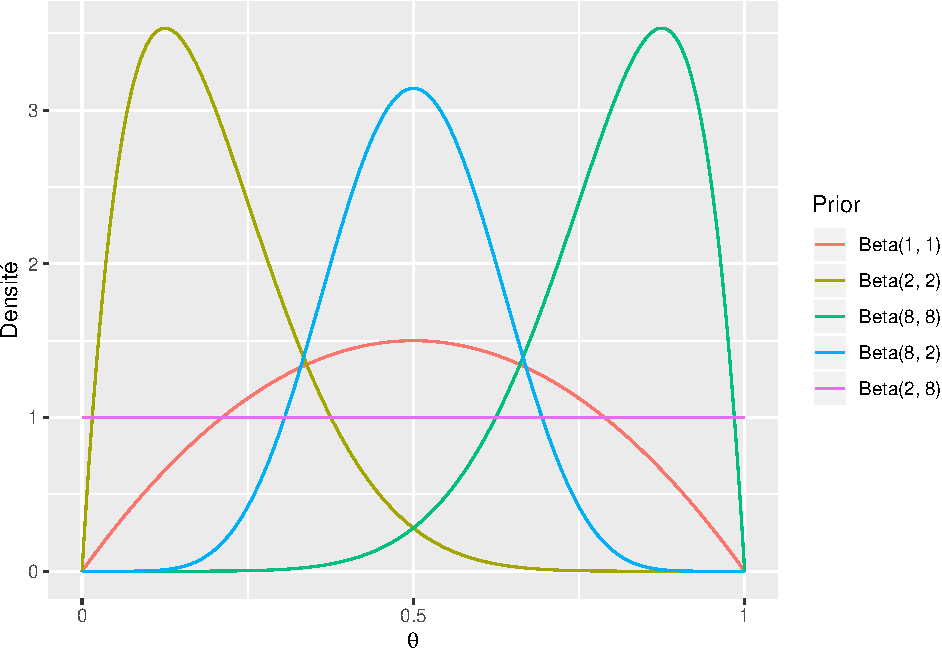
\includegraphics{chapitre_inference_bayesienne_files/figure-latex/df_prior-1.pdf}

L'expression analytique du prior est donc donnée par:
\[\pi(\theta) = \frac {\theta^{a -1}(1-\theta)^{b -1}}{\int _{0}^{1}u^{a -1}(1-u)^{b -1}\,du}\mathbf{1}_{0 < \theta < 1} \propto \theta^{a -1}(1-\theta)^{b -1}\mathbf{1}_{0 < \theta < 1}\]

\hypertarget{loi-a-posteriori}{%
\subsubsection{Loi a posteriori}\label{loi-a-posteriori}}

On cherche la loi de \(\theta \vert \mathbf{X}\).

On a directement que: \begin{align*}
\pi(\theta \vert\mathbf{X}) &\propto L(\mathbf{X}\vert \theta)\pi(\theta)\\
&\propto \theta^{\sum_{k=1}^n X_k}\left(1 - \theta \right)^{n - \sum_{k=1}^n X_k} \theta^{a -1}(1-\theta)^{b -1}\mathbf{1}_{0 < \theta < 1}\\
&\propto \theta^{a + \sum_{k=1}^n X_k - 1}(1-\theta)^{b + n - \sum_{k=1}^n X_k -1}\mathbf{1}_{0 < \theta < 1}
\end{align*} On reconnaît que \(\pi(\theta\vert \mathbf{X})\) est la
densité d'une loi
\[\theta\vert \mathbf{X} \sim \beta\left(a + \underbrace{\sum_{k = 1}^n X_k}_{\text{Nb. piles}},~b + \underbrace{n - \sum_{k = 1}^n X_k}_{\text{Nb. faces}}\right)\]

Le fait que la \emph{loi a posteriori} soit dans la même famille que la
loi \emph{a priori} est une propriété de conjugaison du modèle binomial
avec le prior de loi beta. Ce prior est dit conjugué.

\hypertarget{estimateurs-bayuxe9siens-1}{%
\subsubsection{Estimateurs bayésiens}\label{estimateurs-bayuxe9siens-1}}

\begin{itemize}
\tightlist
\item
  \textbf{Maximum a posteriori (MAP)}
\end{itemize}

On peut montrer que, pour \(a + b + n > 2\) et
\(a + \sum_{k = 1}^n x_k \geq 1\)
\[MAP(\theta \vert \mathbf{X}) = \frac{a + \sum_{k = 1}^n X_k-1}{a  +  b + n -2}\]
On remarque que pour \(a = b = 1\) (prior uniforme), il s'agit du
maximum de vraisemblance, et que pour tout couple \((a, b)\), cette
quantité converge vers le maximum de vraisemblance quand \(n\) grandit.

\begin{itemize}
\tightlist
\item
  \textbf{Espérance a posteriori}
\end{itemize}

Par propriété de la loi \(\beta\), on:
\[\mathbb{E}[\theta \vert \mathbf{X}] \overset{\text{loi } \beta}{=} \frac{a + \sum_{k = 1}^n X_k}{a + b + n} = \underbrace{\frac{n}{a + b + n}}_{\text{Poids données}}\times \overbrace{\frac{\sum_{k=1}^n X_k}{n}}^{\text{Max. de vrais.}} + \underbrace{\frac{a + b}{a + b + n}}_{\text{Poids prior}} \times \overbrace{\frac{a}{a + b}}^{\mathbb{E}\text{ du prior}}\]

Encore une fois, la décomposition illustre le poids des données et le
poids du prior. On remarque que pour \(n\) suffisament grand, tous les
priors seront équivalents.

\begin{itemize}
\tightlist
\item
  \textbf{Régions de crédibilité}
\end{itemize}

Toute région de crédibilité peut facilement être obtenue à l'aide de la
fonction quantile de la loi \(\beta\), qui est implémentée dans tout
logiciel de statistiques.

\hypertarget{posterior-de-loi-inconnue-moduxe8le-de-ruxe9gression-probit}{%
\subsection{Posterior de loi inconnue: modèle de régression
probit:}\label{posterior-de-loi-inconnue-moduxe8le-de-ruxe9gression-probit}}

\hypertarget{pruxe9diction-de-pruxe9sence-doiseaux}{%
\subsubsection{Prédiction de présence
d'oiseaux}\label{pruxe9diction-de-pruxe9sence-doiseaux}}

Une étude consiste en l'observation de la présence ou non de la linotte
mélodieuse sur différents sites échantillonnés.

Sur ces différents sites sont mesurées différentes caractéristiques:

\begin{itemize}
\tightlist
\item
  Le nombre de vers moyens sur une surface au sol de \(1m^2\).
  (Covariable 1)
\item
  La hauteur d'herbe moyenne sur une surface au sol de \(1m^2\).
  (Covariable 2)
\item
  On calcule cette hauteur d'herbe au carré. (Covariable 3).
\end{itemize}

On peut représenter la présence ou non d'oiseaux en fonctions des
caractéristiques du site:

\begin{Shaded}
\begin{Highlighting}[]
\KeywordTok{ggplot}\NormalTok{(donnees_presence, }\KeywordTok{aes}\NormalTok{(}\DataTypeTok{x =}\NormalTok{ haut_herbe, }\DataTypeTok{y =}\NormalTok{ dens_vers)) }\OperatorTok{+}
\StringTok{  }\KeywordTok{geom_point}\NormalTok{(}\KeywordTok{aes}\NormalTok{(}\DataTypeTok{col =}\NormalTok{ presence)) }\OperatorTok{+}\StringTok{ }
\StringTok{  }\KeywordTok{labs}\NormalTok{(}\DataTypeTok{x =} \StringTok{"Hauteur d'herbe"}\NormalTok{, }
       \DataTypeTok{y =} \StringTok{"Densité de vers"}\NormalTok{, }
       \DataTypeTok{col =} \StringTok{"Présence"}\NormalTok{)}
\end{Highlighting}
\end{Shaded}

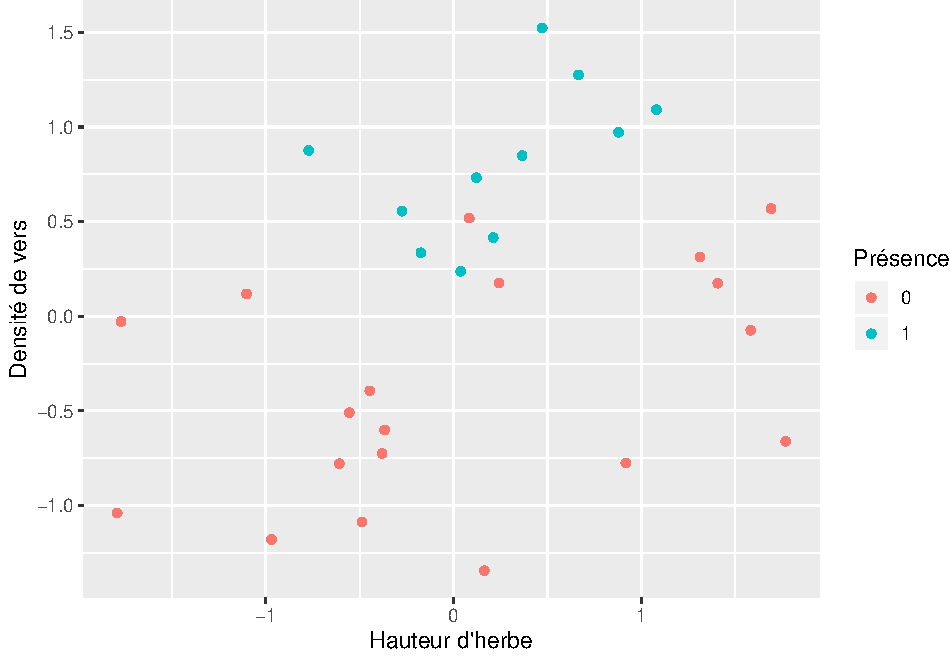
\includegraphics{chapitre_inference_bayesienne_files/figure-latex/plot_donnees_presence-1.pdf}

\hypertarget{notations-et-moduxe8le-de-ruxe9gression-probit}{%
\subsubsection{Notations et modèle de régression
probit}\label{notations-et-moduxe8le-de-ruxe9gression-probit}}

On note \(y_1, \dots, y_n\) les observations de présence (1 si on
observe un oiseau, 0 sinon) sur les sites \(1\) à \(n\).

On note
\[\mathbf{x}_k = (\overset{\text{Nb. vers}}{x_{k,1}}, \overset{\text{Haut. herbe}}{x_{k,2}}, \overset{\text{Haut. herbe}^2}{x_{k,3}})^T\]
le vecteur des covariables sur le \(k\)-ème site \((1\leq k \leq n)\).

On pose le modèle suivant:

\(Y_k \sim \mathcal{B}ern(p_k)\) où
\[p_k = \phi(\beta_0 + \beta_1 x_{i1} + \beta_2x_{i2} + \beta_3 x_{i3}) = \phi(\mathbf{x}_k^T\theta),\]
où

\begin{itemize}
\tightlist
\item
  \(\phi\) est la fonction de répartition d'une \(\mathcal{N}(0, 1)\),
  i.e.
  \[\phi(z) = \frac{1}{\sqrt{2\pi}}\int_{-\infty}^z \text{e}^{-\frac{u^2}{2}}\text{d}u\]
\item
  \(\theta = \left\lbrace \beta_0, \beta_1, \beta_2, \beta_3\right\rbrace\)
  est le vecteur des paramètres à estimer.
\end{itemize}

\hypertarget{vraisemblance}{%
\subsubsection{Vraisemblance}\label{vraisemblance}}

Pour un vecteur d'observations \(\mathbf{Y} = Y_{1:k}\), la
vraisemblance
\[L(\mathbf{Y}\vert \theta) = \prod_{k = 1}^n \underset{\text{Proba. présence}}{\phi(\mathbf{x}_k^T\theta)^{Y_k}}\times \underset{\text{Proba. absence}}{(1 - \phi(\mathbf{x}_k^T\theta))}^{1 - Y_k}\]

\hypertarget{prior-sur-theta}{%
\subsubsection{\texorpdfstring{Prior sur
\(\theta\)}{Prior sur \textbackslash{}theta}}\label{prior-sur-theta}}

Comme a priori sur \(\theta\), on choisit une normale avec une grande
variance\(\theta \overset{\text{prior}}{\sim} \mathcal{N}(0, 4 I),\)
donc
\[\pi(\theta) = \frac{1}{\sqrt{2\pi \times 4}^4} \text{e}^{-\frac{1}{8}\theta^T\theta}\]
où \(I\) est la matrice Identité (ici \(4 \times 4\))

\hypertarget{posterior}{%
\subsubsection{Posterior}\label{posterior}}

Le posterior est donc donné par:
\[\pi(\theta \vert \mathbf{Y}) \propto \pi(\theta) L(\mathbf{Y}\vert \theta) \propto \frac{1}{64\pi^2}\text{e}^{-\frac{1}{8}\theta^T\theta} \prod_{k = 1}^n \phi(\mathbf{x}_k^T\theta)^{Y_k} (1 - \phi(\mathbf{x}_k^T\theta))^{1 - Y_k}\]

Cette densité n'est pas standard. Ainsi, on ne connaît pas ces
caractéristiques associées et intéressantes (quantiles, espérance,
variance). Ces différentes quantités peuvent cependant être approchées
par méthode de Monte Carlo, si tant est qu'on soit capable de simuler
selon cette loi.

\hypertarget{simulation-duxe9chantillons-a-posteriori-par-acceptation-rejet}{%
\subsubsection{Simulation d'échantillons a posteriori par acceptation
rejet}\label{simulation-duxe9chantillons-a-posteriori-par-acceptation-rejet}}

Notre objectif est de simuler selon le posterior défini ci dessus. On va
pour ce faire procéder par méthode d'acceptation rejet.

On remarque immédiatement qu'on ne peut pas utiliser l'acceptation rejet
classique, car \(\pi(\theta \vert \mathbf{Y})\) n'est connu qu'à une
cnstante près!

Cependant, si on note
\[\tilde{\pi}(\theta \vert \mathbf{Y}) = \frac{1}{64\pi^2}\text{e}^{-\frac{1}{8}\theta^T\theta} \prod_{k = 1}^n \phi(\mathbf{x}_k^T\theta)^{Y_k} (1 - \phi(\mathbf{x}_k^T\theta))^{1 - Y_k},\]
on peut utiliser la propriété vue en TD, qui dit qu'il suffit de
connaître \(\tilde{\pi}\) pour simuler selon \(\pi\) à partir
d'acceptation rejet.

\begin{itemize}
\tightlist
\item
  \textbf{Choix de la densité de proposition}
\end{itemize}

Comme densité de proposition, on peut par exemple prend pour \(g\) la
densité correspondant au prior (\(g(\theta) = \pi(\theta)\)). On
remarque que dans ce cas
\[\frac{\tilde{\pi}(\theta \vert \mathbf{Y})}{g(\theta)} = \frac{\pi(\theta)L(\mathbf{Y}\vert \theta)}{\pi(\theta)} = \prod_{k = 1}^n \phi(\mathbf{x}_k^T\theta)^{Y_k} (1 - \phi(\mathbf{x}_k^T\theta))^{1 - Y_k} \leq 1 =:M.\]

On a donc un majorant uniforme en \(\theta\) et l'acceptation rejet
suivant permet de tirer selon \(\pi(\theta \vert \mathbf{Y})\):

\begin{enumerate}
\def\labelenumi{\arabic{enumi}.}
\tightlist
\item
  On tire \(\theta_{cand} \sim \mathcal{N}(0, 4I)\)
\item
  On tire (independamment) \(U\sim \mathcal{U}[0, 1]\)
\item
  Si \(U < \frac{L(y_{1:n}\vert \theta)}{M}\), on accepte
  \(\theta_{cand}\)
\item
  Sinon on recommence
\end{enumerate}

\hypertarget{echantillon-du-posterior-loi-a-posteriori-marginales-et-estimateurs-bayuxe9siens}{%
\subsubsection{Echantillon du posterior, loi a posteriori marginales et
estimateurs
bayésiens}\label{echantillon-du-posterior-loi-a-posteriori-marginales-et-estimateurs-bayuxe9siens}}

\begin{itemize}
\tightlist
\item
  \textbf{Lois marginales}
\end{itemize}

On effectue un tirage de taille \(M = 1000\). On peut représenter la
densité empirique de cet échantillon

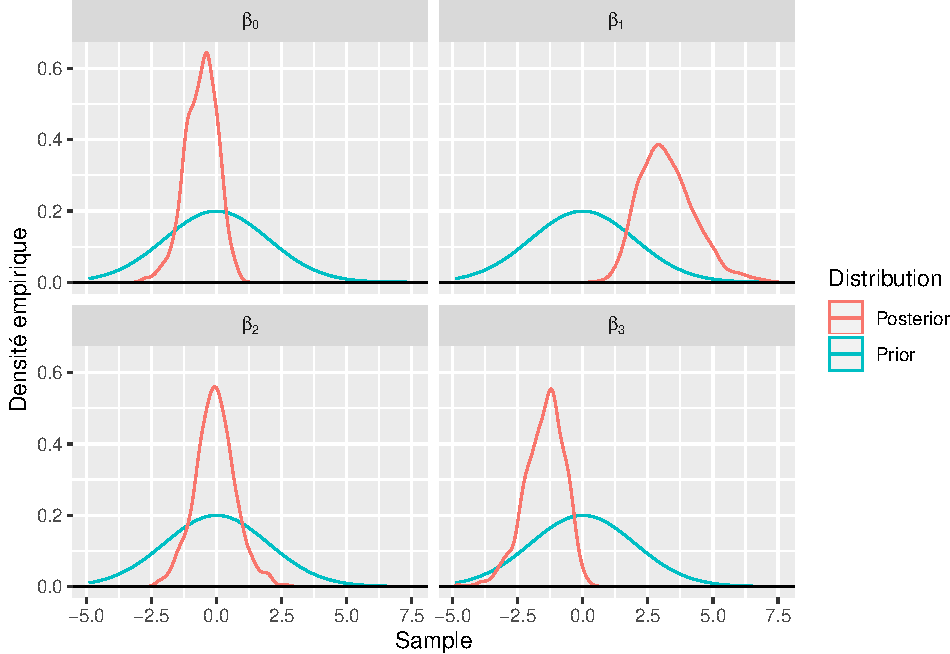
\includegraphics{chapitre_inference_bayesienne_files/figure-latex/plot_posterior_samples-1.pdf}

On peut remarquer que les densités du posterior sont différentes du
prior.

\begin{itemize}
\tightlist
\item
  \textbf{Loi jointe}
\end{itemize}

Il peut être intéressé de regarder la loi jointe obtenue par simulation.
On pourra notamment remarquer qu'un prior indépendant sur les
composantes n'entraîne pas une indépendance dans le posterior. Par
exemple, on représente ici la loi du couple
\((\beta_0,\beta_1 \vert \mathbf{Y})\):

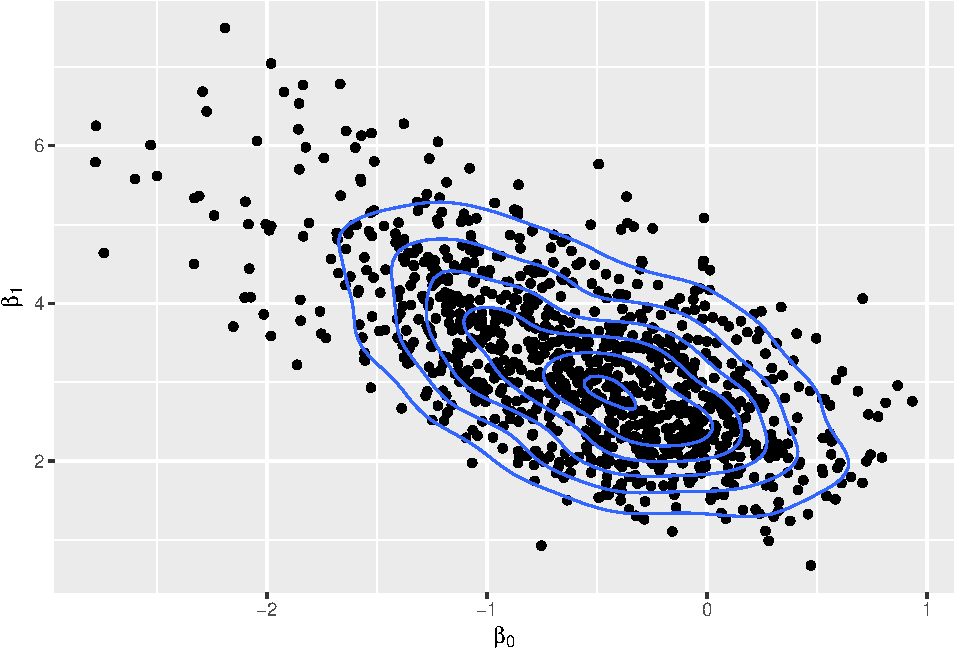
\includegraphics{chapitre_inference_bayesienne_files/figure-latex/loi_jointe_beta0_beta1-1.pdf}

On voit qu'il existe une correlation linéaire négative entre ces deux
variables aléatoires, qui étaient, a priori, supposées indépendantes.

\begin{itemize}
\tightlist
\item
  \textbf{Espérance a posteriori et intervalles de crédibilité}
\end{itemize}

Comme on sait simuler selon la loi cible, les espérances peuvent être
approchées par méthode de Monte Carlo classique. On obtient ici une
estimation del'espérance \textbf{a posteriori} ainsi qu'un intervalle de
confiance a posterirori

\begin{longtable}[]{@{}lrrr@{}}
\toprule
Paramètre & Esperance a posteriori. & Quantile 2.5\% & Quantile
97.5\%\tabularnewline
\midrule
\endhead
beta{[}0{]} & -0.586 & -1.980890 & 0.5264341\tabularnewline
beta{[}1{]} & 3.250 & 1.538387 & 5.7005273\tabularnewline
beta{[}2{]} & -0.051 & -1.554202 & 1.5786397\tabularnewline
beta{[}3{]} & -1.477 & -3.171951 & -0.2424187\tabularnewline
\bottomrule
\end{longtable}

\hypertarget{au-deluxe0-de-lacceptation-rejet}{%
\subsection{Au delà de l'acceptation
rejet}\label{au-deluxe0-de-lacceptation-rejet}}

Dans le cas précédent, l'espérance du temps d'attente avant une
acceptation est donnée par
\[\frac{M}{\int L(\mathbf{Y}\vert \theta)\pi(\theta) \text{d}\theta}\]

Mécaniquement, cette quantité augmente quand \(n\) augmente, et
l'acceptation rejet dvient prohibitif.

En pratique, l'inférence Bayésienne utilisera d'autres algorithmes de
simulations de loi: les algorithmes de Monte Carlo par chaîne de Markov.


\end{document}
